\section{Basic Graph Concepts}

\begin{quote}
    A graph G = (V, E) consists of a set of nodes (vertices) V and a set of edges E
\end{quote}
    
%\end{displayquote}

Each edge connects two nodes and represents the relationship between the two nodes. Graphs can be directed (edges have a direction) as shown in Figure \ref{Directed_Graph} (page \pageref{Directed_Graph}) or undirected (edges have no direction) as shown in Figure \ref{Undirected_Graph} (page \pageref{Undirected_Graph}). Additionally, graphs can be weighted, where edges have an associated weight representing the strength of the connection between the nodes. 

%insert image of an undirected and a directed graph

\begin{figure}
     \centering
     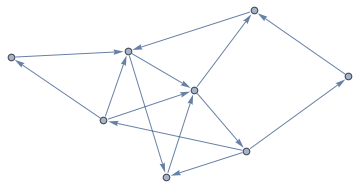
\includegraphics[width= 0.4\textwidth]{pics/Directed_Graph.png}
     \caption{Directed Graph}
     \label{Directed_Graph}
\end{figure}

\begin{figure}
     \centering
     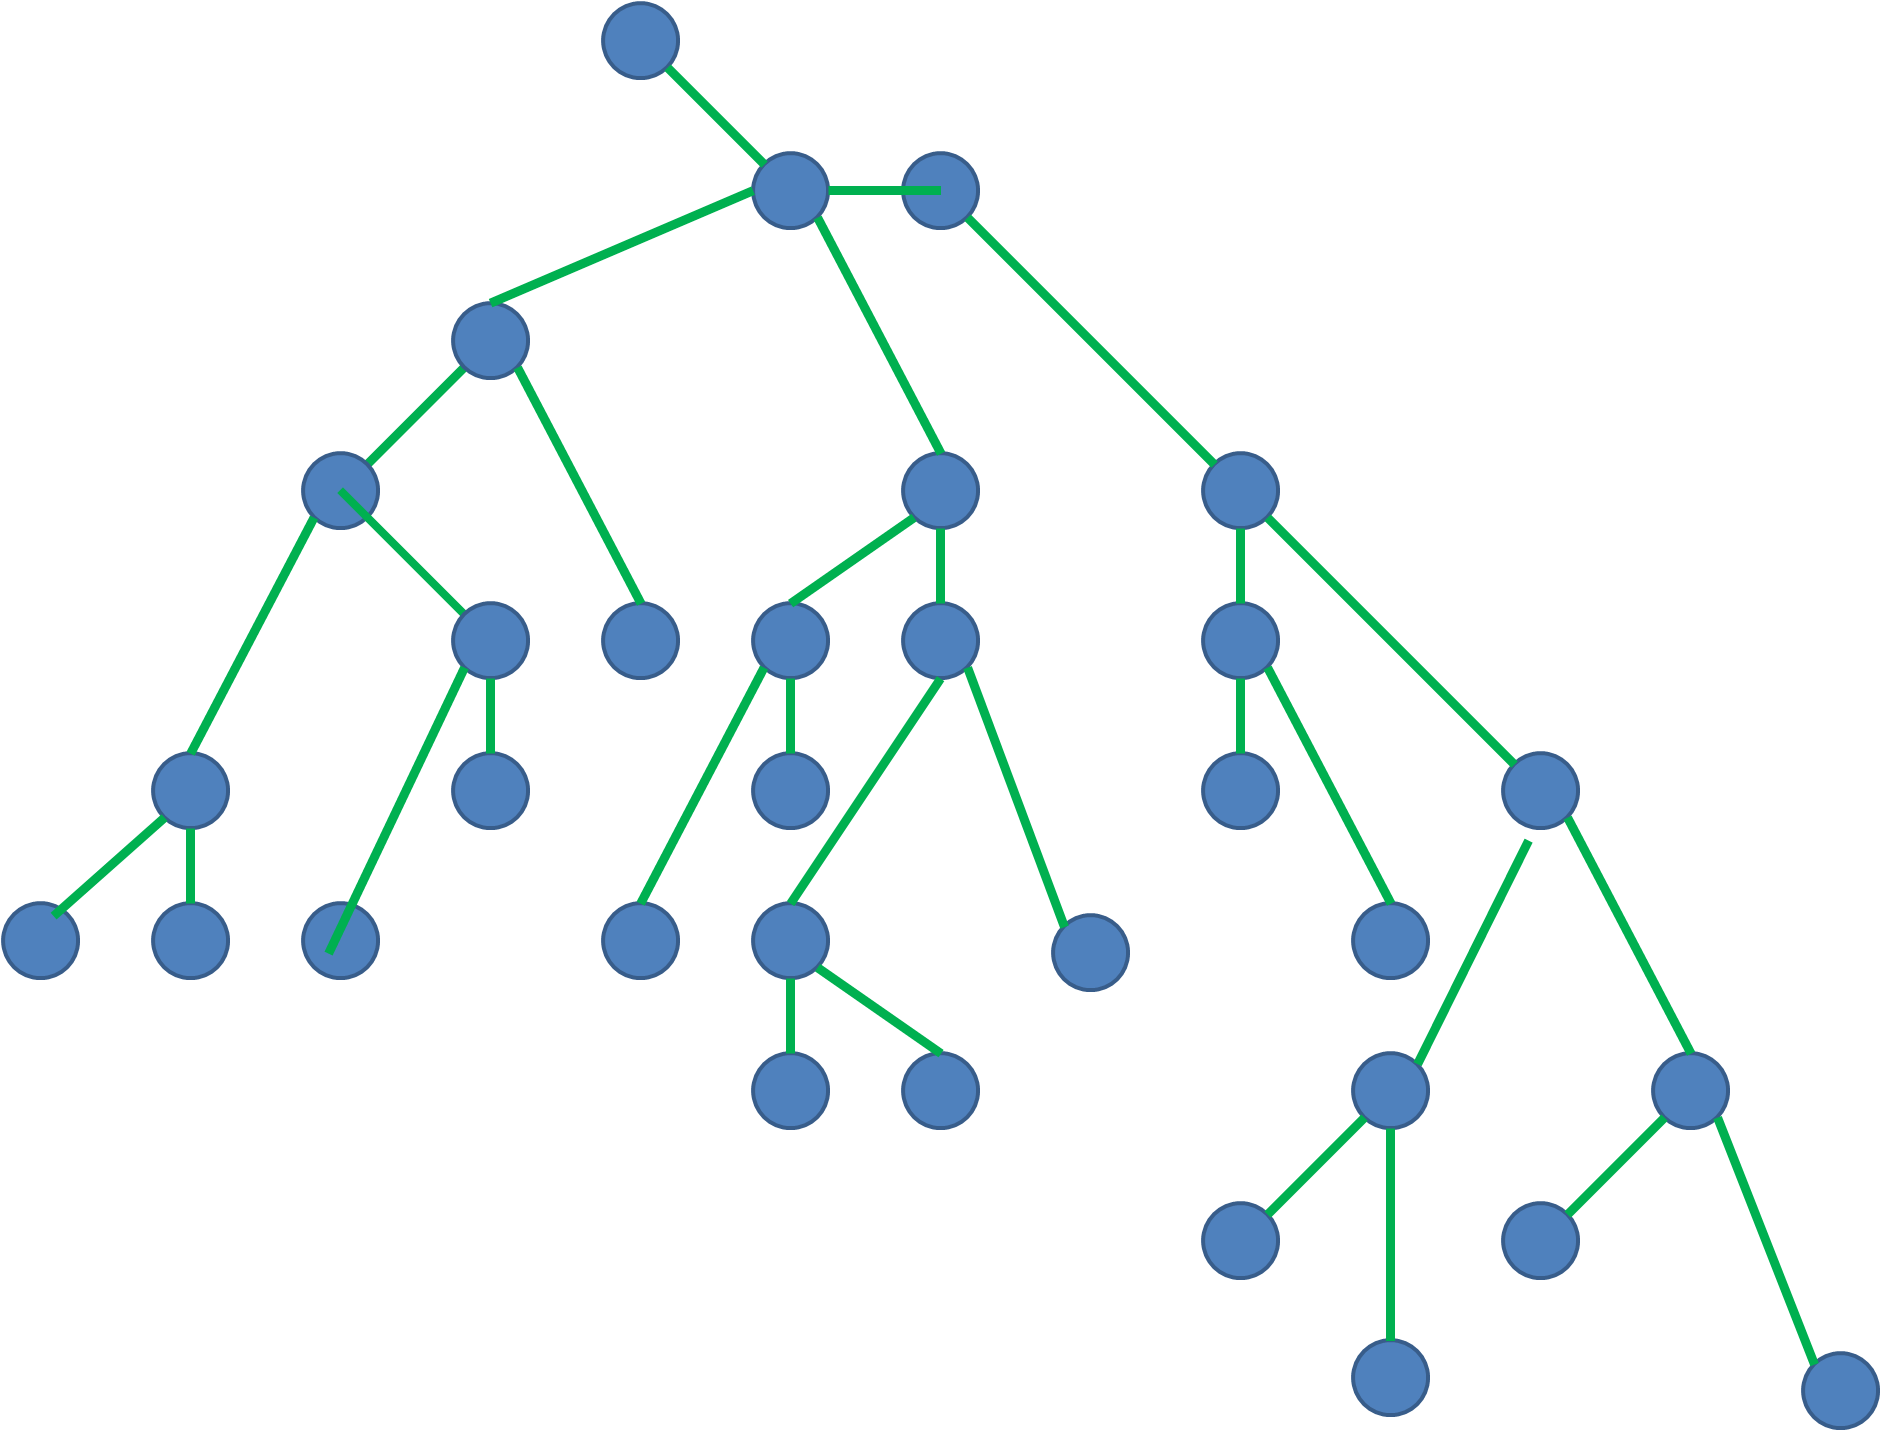
\includegraphics[width= 0.4\textwidth]{pics/Undirected_Graph.png}
     \caption{Undirected Graph}
     \label{Undirected_Graph}
\end{figure}

Graphs are represented using the adjacency matrix A where each element in the matrix $A_{ij}$ represent the weight of edge from $node_i$ to $node_j$.

%give the example adjacency matrix for a small graph's node

A degree of node can be defined as the number of neighbour nodes $N(v)$. 

\begin{quote}
    Note : \textit{Nodes} and \textit{edges} are very general terms and can mean a lot of things. For example, a node itself could be a Deep Neural Network and an edge could represent a producer-consumer relationship, evolutionary relationship, a chemical bond, a dataflow relationship or even a mechanical connection.
\end{quote}

\subsection{Modelling Using Graphs}
%\begin{quote}
Graphs allow for the most flexible and accurate representation of a lot of modelling problems. In general, engineering involves the creation of a model with certain (reasonable) assumptions. The objective of creating a model is to ultimately utilise the model for its predictive capabilities. Thus, the modelling framework or approach we take, influences both the way we see a problem and also its solution. A good number of problems that we are trying to solve can be represented as a graph model - 
\begin{enumerate}
    \item Social Media Networks - where every individual is modelled as node and their relation is the edge between them 
    \item Molecules - Every atom is a node and the bond between them is an edge
    \item Proteins - Proteins are represented as a graph (G) of Aminoacids (N) connected to each other by an edge (E)
\end{enumerate}

%\subsection{General Recipe}
So, the basic recipe for a GNN is
\begin{enumerate}
  %\item Identify the graph structure that you want to apply GNN on i.e, formulate the nodes and edges in the data.
  \item Construct the initial graph structure to model the data as nodes and the relationship between data as edges
  \item Based on the task i.e, node level, edge level as described earlier, create the GNN model's classification layer
  \item Define the loss function according to the context. Eg: log likelihood, root mean square error etc.
  \item Apply gradient descent and optimize the weight parameters by minimizing the loss function
\end{enumerate}